\documentclass[12pt]{article}
\usepackage[top=1in,bottom=1in,left=1in,right=1in]{geometry}
\usepackage{alltt}
\usepackage{array}	
\usepackage{graphicx}
\usepackage{tabularx}
\usepackage{verbatim}
\usepackage{setspace}
\usepackage{listings}
\usepackage{amssymb,amsmath, amsthm}
\usepackage{qtree}
\usepackage{hyperref}
\usepackage{oz}
\usepackage[cc]{titlepic}
\usepackage{fancyvrb}
\usepackage{epstopdf}
\usepackage{soul}
\usepackage{array}
\usepackage{graphicx}
\graphicspath{ {./images/} }
\newcolumntype{L}{>{\centering\arraybackslash}m{3cm}}
\usepackage[affil-it]{authblk}

% title
\title{SOEN 331: Introduction to Formal Methods for Software Engineering \\
\textbf{Assignment 4} \\
Temporal Logic}

\author{Duc Nguyen - 40064649\\
        Vithura Muthiah - 40062305\\
        Auvigoo Ahmed - 40128901\\
        Ali Hanni - 40157164}
 \affil{Gina Cody School of Computer Science and Software Engineering \\
    Concordia University, Montreal, QC, Canada}
\date{Winter 2021}

\begin{document}
\maketitle

\newpage
\tableofcontents

\newpage
\section{Problem 1: Analyzing program behavior}

\text{The behavior of a program is expressed by the following temporal formula:}

% Start section
\begin{figure}[h!]
	\centering 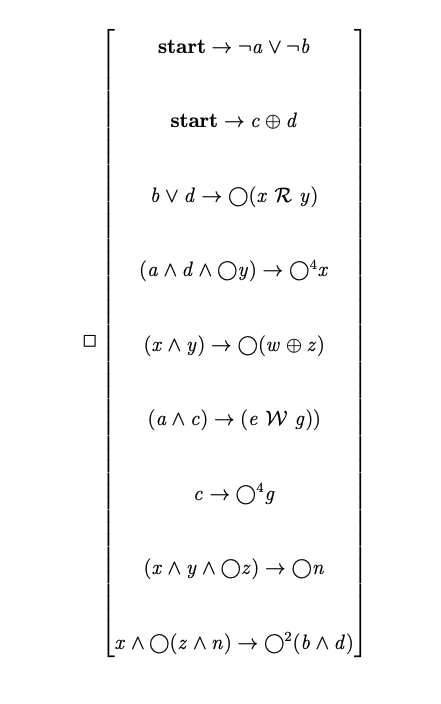
\includegraphics[width=0.8\textwidth]{Problem1Formula}
\end{figure}

\newpage
\subsection{Visualize}

\text{Visualize all models of behavior.}
\subsection{Specify conditions}

\text{There are three models whereby the program terminates:}

\begin{enumerate}
    \item $\langle (a \wedge c \wedge e), e, e, e, g \rangle $
    \item $\langle (a \wedge d), y, y, y, (y \wedge x), w  \rangle $
    \item $\langle c, g \rangle $
\end{enumerate}

\newpage
\section{Problem 2: Visualizing temporal expressions}

\text{Provide a description and a visualization of each of the following expressions:}

\subsection{}

\begin{itemize}
   \item[] $\square \phi \rightarrow \diamond \psi$ 
\end{itemize}

\subsection{}

\begin{itemize}
   \item[] $\square \phi \rightarrow \bigcirc \square \diamond \psi$ 
\end{itemize}

\indent $\phi$ is always true at all times, while $\psi$ will eventually always become true (it can be happen next or in some future moment).

\begin{figure}[h!]
	\centering 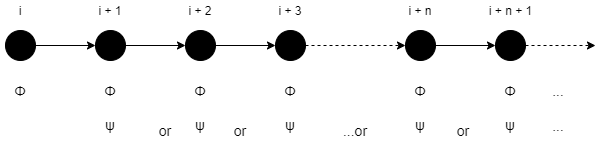
\includegraphics[width=0.8\textwidth]{Problem2-2}
\end{figure}
\subsection{}

\begin{itemize}
   \item[] $(\phi \land \bigcirc \psi) \rightarrow \diamond \square \tau$ 
\end{itemize}
\subsection{}

\begin{itemize}
   \item[] $(\psi \land \bigcirc \chi) \rightarrow \bigcirc \tau$ 
\end{itemize}


\noindent $\psi$ is true at time i and $\chi$ will be true at the very next state (i+1), while $\tau$ will
be true at the next state (i+1). 

\begin{figure}[h!]
	\centering 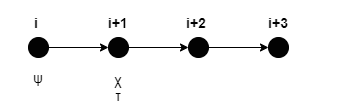
\includegraphics[width=0.8\textwidth]{Problem2-4}
\end{figure}
\subsection{}

\begin{itemize}
   \item[] $(\chi \land \bigcirc \omega) \rightarrow \bigcirc^{2} (\phi \textbf{U} \psi)$ 
\end{itemize}
\subsection{}

\begin{itemize}
   \item[] $(\phi \oplus \psi) \rightarrow \square \omega$ 
\end{itemize}

\noindent Either $\phi$ or $\psi$ are true at time i (but never both), while $\omega$ is always true.

\begin{figure}[h!]
	\centering 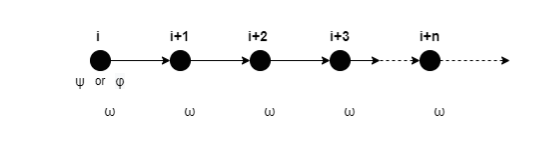
\includegraphics[width=0.8\textwidth]{Problem2-6.png}
\end{figure}
\subsection{}

\begin{itemize}
   \item[] $\chi \land \bigcirc (\chi \land \psi) \rightarrow \diamond \omega$
\end{itemize}
\subsection{}

$
\begin{bmatrix}
(\chi \land \bigcirc^{2} \psi) \rightarrow \bigcirc^{2} (\tau \textbf{W} \omega) \\
\mu \rightarrow \bigcirc^{5} \omega
\end{bmatrix}
$

\end{document}
